\documentclass[9pt, twocolumn]{extarticle}
\usepackage{amsmath,amssymb,amsfonts}
\usepackage{graphicx,color}
\usepackage{xcolor}
\usepackage{tikz}

\begin{document}

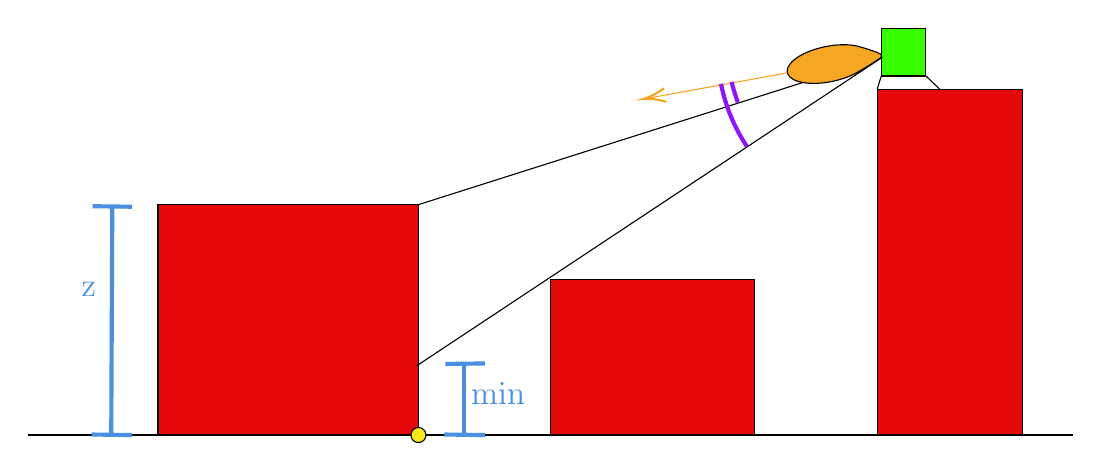
\begin{tikzpicture}[x=0.75pt,y=0.75pt,yscale=-1,xscale=1]

\draw  [fill={rgb, 255:red, 228; green, 8; blue, 8 }  ,fill opacity=1 ] (459,83.5) -- (529,83.5) -- (529,250) -- (459,250) -- cycle ;
\draw    (50,250) -- (553.33,250) ;
\draw  [fill={rgb, 255:red, 55; green, 255; blue, 0 }  ,fill opacity=1 ] (461,54) -- (482.5,54) -- (482.5,77) -- (461,77) -- cycle ;
\draw  [fill={rgb, 255:red, 228; green, 8; blue, 8 }  ,fill opacity=1 ] (112.5,139) -- (238,139) -- (238,250) -- (112.5,250) -- cycle ;
\draw  [fill={rgb, 255:red, 228; green, 8; blue, 8 }  ,fill opacity=1 ] (301.5,175) -- (400,175) -- (400,250) -- (301.5,250) -- cycle ;
\draw    (461.5,68) -- (237,216.75) ;
\draw    (482.5,77) -- (489.5,83.75) ;
\draw    (461,77) -- (459,83.5) ;
\draw    (238,139) -- (461.5,68) ;
\draw [color={rgb, 255:red, 74; green, 144; blue, 226 }  ,draw opacity=1 ][fill={rgb, 255:red, 0; green, 76; blue, 255 }  ,fill opacity=1 ][line width=1.5]    (260,215.88) -- (260,249.63) ;
\draw [color={rgb, 255:red, 74; green, 144; blue, 226 }  ,draw opacity=1 ][fill={rgb, 255:red, 0; green, 76; blue, 255 }  ,fill opacity=1 ][line width=1.5]    (251,215.75) -- (270,215.5) ;
\draw [color={rgb, 255:red, 74; green, 144; blue, 226 }  ,draw opacity=1 ][line width=1.5]    (90.5,140) -- (90,250) ;
\draw [color={rgb, 255:red, 74; green, 144; blue, 226 }  ,draw opacity=1 ][fill={rgb, 255:red, 0; green, 76; blue, 255 }  ,fill opacity=1 ][line width=1.5]    (250.5,249.75) -- (270,250) ;
\draw [color={rgb, 255:red, 74; green, 144; blue, 226 }  ,draw opacity=1 ][fill={rgb, 255:red, 0; green, 76; blue, 255 }  ,fill opacity=1 ][line width=1.5]    (81,139.75) -- (100,140) ;
\draw [color={rgb, 255:red, 74; green, 144; blue, 226 }  ,draw opacity=1 ][fill={rgb, 255:red, 0; green, 76; blue, 255 }  ,fill opacity=1 ][line width=1.5]    (80.5,249.75) -- (100,250) ;
\draw  [fill={rgb, 255:red, 248; green, 231; blue, 28 }  ,fill opacity=1 ] (234.38,250.25) .. controls (234.25,248.25) and (235.75,246.52) .. (237.75,246.38) .. controls (239.75,246.25) and (241.48,247.75) .. (241.62,249.75) .. controls (241.75,251.75) and (240.25,253.48) .. (238.25,253.62) .. controls (236.25,253.75) and (234.52,252.25) .. (234.38,250.25) -- cycle ;
\draw [color={rgb, 255:red, 245; green, 166; blue, 35 }  ,draw opacity=1 ]   (461.07,67.28) -- (348.11,87.79) ;
\draw [shift={(346.14,88.14)}, rotate = 349.71] [color={rgb, 255:red, 245; green, 166; blue, 35 }  ,draw opacity=1 ][line width=0.75]    (10.93,-3.29) .. controls (6.95,-1.4) and (3.31,-0.3) .. (0,0) .. controls (3.31,0.3) and (6.95,1.4) .. (10.93,3.29)   ;
\draw  [fill={rgb, 255:red, 245; green, 166; blue, 35 }  ,fill opacity=1 ] (449.49,75.24) .. controls (449.49,75.24) and (449.49,75.24) .. (449.49,75.24) .. controls (441.46,79.89) and (428.77,81.88) .. (421.14,79.68) .. controls (413.52,77.47) and (413.85,71.92) .. (421.88,67.27) .. controls (429.91,62.62) and (442.6,60.63) .. (450.22,62.83) .. controls (458.46,65.21) and (462.08,66.7) .. (461.07,67.28) .. controls (462.02,67.56) and (458.16,70.22) .. (449.49,75.24) -- cycle ;
\draw  [draw opacity=0][line width=1.5]  (396.21,110.88) .. controls (395.21,109.38) and (394.25,107.83) .. (393.34,106.24) .. controls (388.65,98.09) and (385.5,89.49) .. (383.79,80.78) -- (461.07,67.28) -- cycle ; \draw  [color={rgb, 255:red, 144; green, 19; blue, 254 }  ,draw opacity=1 ][line width=1.5]  (396.21,110.88) .. controls (395.21,109.38) and (394.25,107.83) .. (393.34,106.24) .. controls (388.65,98.09) and (385.5,89.49) .. (383.79,80.78) ;  
\draw  [draw opacity=0][line width=1.5]  (391.86,89.65) .. controls (390.67,86.42) and (389.68,83.16) .. (388.89,79.89) -- (461.07,67.28) -- cycle ; \draw  [color={rgb, 255:red, 144; green, 19; blue, 254 }  ,draw opacity=1 ][line width=1.5]  (391.86,89.65) .. controls (390.67,86.42) and (389.68,83.16) .. (388.89,79.89) ;  

% Text Node
\draw (262.01,223.38) node [anchor=north west][inner sep=0.75pt]  [font=\large,rotate=-0.23,xslant=-0.01] [align=left] {\textcolor[rgb]{0.29,0.56,0.89}{min}};
% Text Node
\draw (74.47,174.93) node [anchor=north west][inner sep=0.75pt]  [font=\large,rotate=-0.23,xslant=-0.01] [align=left] {\textcolor[rgb]{0.29,0.56,0.89}{z}};
\end{tikzpicture}

\end{document}